\chapter{Introduction} \label{chap:introduction}
\par
Modern information and communication technologies are widely used in almost every field.  It has also influenced the environmental science. Using the power of the new technologies, it is possible to create high quality models, simulations and decision support systems to help environmental scientists improve their research. Environmental modelling is the simplified view of the complex environmental realities. It represents the environmental objects, natural phenomena and physical processes in a logical way. It formalizes the principles of natural sciences to interpret the natural reality. Nowadays, modelling the complex environmental phenomena remains a great challenge. We need to consider the different dimensions and amount of data, structures of different sub components, scalability and adaptability of our models.
\par
These requirements have led to the development of different environmental modelling frameworks, such as CCA, ESMF, TIME, OMS, etc. These frameworks are implemented in general purpose languages, such as C, Java, Fortran, etc. They mostly provide application programming interfaces, which were specially implemented according to the needs of environmental modelling. They help the scientists to develop, adapt, reuse or integrate different models. However, they carry with them many kinds of disadvantages. Software implementations of environmental models are seldom reused by broader communities or in different modelling frameworks, because of the poor semantic of the model interfaces. In most cases, the models are only usable for a specific application. It is hard for other components to make use of the available models, because of the poor communication abilities of the models.
\par
To overcome the disadvantages of the available model frameworks, domain specific language brings about a lot of benefits. It offers appropriate domain specific syntax and notations, which allows the user to describe a solution at the level of abstraction of the problem domain. It allows validation at the domain level. Environmental scientists can make the best use of the domain specific language, because it follows the domain abstractions and semantics as closely as possible. The build-in functions like analysis, verification, optimization, parallelization and  transformation allow the scientists to create reliable models with high quality and productivity, which are easy to maintain and distribute on other platforms.
\par
The following section describes the project goals which aims to solve these problems. Furthermore, the various features of the solution will be described in the section \nameref{sec:vision_for_a_dsl}. After that the priorities of the project goals will be defined.

\section{Project Goals}
\par
The main goal of the project is a feasibility study for a more universal approach to describe environmental models. A domain specific language was proposed as a solution to this need. Although, a plain DSL will not be enough to solve all problems involved in describing an environmental model in such ways that it can be fully described and exchanged without additional information. The following features were defined by Athanasiadis [cite] as necessary for a language or system that allows to fully describe and exchange these environmental models.
\begin{itemize}
	\item Domain-specific data structures
	\item Rich model interfaces    
	\item DSL handling typical operations
	\item Support for different modeling paradigms and frameworks
	\item Account for modeling uncertainty    
	\item Model transparency and defensibility of results 
\end{itemize}
The next section describes the DSL features in more detail.

\section{Vision for a DSL} \label{sec:vision_for_a_dsl}


\subsection{Domain-specific data structures}
\par
Domain-specific data structures can be used by the modeler to semantically describe the following elements in the DSL.
\begin{itemize}
	\item    units and quantities
	\item    accuracy
	\item    spatial and temporal scales and extents
	\item    quality and provenance information of data sources and results
\end{itemize}
\par
The newly created models will consist of independent logical models and their observations. This is a novel approach, as it is a semantical representation of environmental data sets. In other words, the code for one entity is logically capsulated and separated from other entities.
\par
The main idea to achieve this, is to connect the DSL with specific environmental modelling ontologies, as these define the semantics of the environmental terminology.

\subsection{Rich model interfaces}
\par
Rich model interfaces should allow the modeler to share their models in scientific workflows. Therefore the models must be enriched with the following metadata in machine-readable formats.
\begin{itemize}
	\item incorporating model assumptions
	\item pre- and post- conditions
	\item prerequisites for reuse
\end{itemize}

\subsection{DSL handling typical operations}
\par
To simplify the modelers work the DSL should be able to automate typical operations, among this:
\begin{itemize}
	\item scaling
	\item averaging
	\item interpolation
	\item unit conversions
\end{itemize}
\par
The language will be able to treat appropriately intensive and extensive quantities, for example by calculating the weighted mean when joining two intensive quantities.

\subsection{Support for different modeling paradigms and frameworks}
\par
Athanasiadis proposed that the DSL should be paradigm agnostic and should also be able to be compatible to several frameworks. Nevertheless this point makes the development of the DSL very complex. Therefore a focus was set on the System Dynamics paradigm.

\subsection{Account for modeling uncertainty}
\par
The model environment should be able to compute the modeling uncertainty and quality information. This should be achieved with confidence intervals, which solve different sources of uncertainty like:
\begin{itemize}
	\item random sampling error and biases
	\item noisy or missing data
	\item approximation techniques for equation
\end{itemize}
\par
An example would be the standard error propagation. Two variables $x$ and $y$ are given, their mean and variance are represented by the following tuples $(\mu x , \sigma x )$ and $(\mu y , \sigma y )$. If their difference is calculated and saved in $z$, the mean and variance of $z$ is automatically represented in the tuple  $(\mu x - \mu y , \sigma x + \sigma y)$.
\\
Despite the importance of this feature, it was out of the scope of this project and no further investigations were made.

\subsection{Model transparency and defensibility of results}
One feature of the environment should be model transparency and defensibility  to explain the results of the model. This means that for each model output a history of operations on primal sources, enabled by the enrichment of metadata, must exist.

\section{Priorities}
\par
After the first step of information gathering the group decided to organize these features by prioritisation and practicability to proof which goals are achievable in the given time.  
The following order was defined:
\subsection*{Priority 1:}
\begin{itemize}
	\item Domain-specific data structures
	\item DSL definition with typical operations
\end{itemize}
\subsection*{Priority 2:}
\begin{itemize}
	\item  Rich model interfaces
	\item  Model transparency and defensibility of results
\end{itemize}
\subsection*{Priority 3:}
\begin{itemize}
	\item Support for different modeling paradigms and frameworks
	\item Account for modeling uncertainty
\end{itemize}
\par
As a result of the lack of  modelling experience in general and especially the lack of experience with modeling environments it was not possible to implement a DSL that fulfills the above mentioned requirements immediately. The idea was to look at existing modelling frameworks in a first step and afterwards to implement lightweight and easy to understand models with these frameworks to gain experience in modeling on the one hand and to investigate them on strengths and weaknesses on the other hand. Based on this knowledge it should be much easier to define a DSL which integrates the required features. The next chapter gives a rough overview of existing modelling frameworks and examines its strengths and weaknesses regarding the needed features.

\section{Existing Environmental Modelling Frameworks}

\subsection{Similie}

\subsection{ESMF}
\par
The Earth System Modeling Framework (ESMF) is an open source project. It is build upon a scalable, flexible paradigm for building and coupling weather, climate, and other Earth science models. ESMF is based on principles of component-based software engineering \autocite{dsl:esmf-homepage}. The components within an ESMF software application usually represent large-scale physical domains such as the atmosphere, ocean, cryosphere or land surface. The framework includes regridding tools for composing complex, coupled modeling systems, and data structures and utilities for developing individual models \autocite{dsl:esmf-free_lib}.
\par
ESMF provides a complete set of Fortran interfaces and some C and C++ interfaces \autocite{dsl:esmf-tutorial1}. The view of the framework consists of two layers, an infrastructure of utilities and data structures for creating model components, and a superstructure for coupling them. User code is placed between these two layers, to make calls to the infrastructure libraries and be scheduled and synchronized by the superstructure, shown in the Figure \ref{fig:esmf_architecture} \autocite{dsl:esmf-overview}.
\begin{figure}[h]
	\centering
	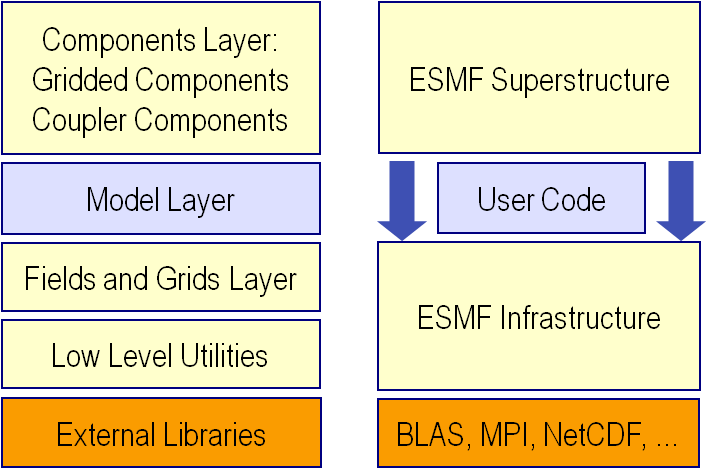
\includegraphics[width=0.7\textwidth]{pics/esmf/esmf_architecture.png}
	\caption[Schematic of the ESMF architecture]{Schematic of the ESMF architecture \autocite{dsl:esmf-regridding} \label{fig:esmf_architecture}}	
\end{figure}
\par
Like many other frameworks, this also does not provide “instructions” that can be used immediately to develop a DSL. To create own models, knowledge in general-purpose languages is required.

\subsubsection {Properties of the modeling}
\par
The ESMF Application Programming Interface (API) is based on the object-oriented programming concept of a class. The major classes in the ESMF superstructure are Components, which typically represent large pieces of functionality such as models, model couplers, dynamics and physics packages, and States, which are the data structures used to communicate data between Components \autocite{dsl:esmf-overview}. User data is represented in the form of data objects such as grids, fields, and arrays. The user can reference a Fortran array to an ESMF array or field, or retrieve a Fortran array out of an ESMF array or field. The fields on the same grid can be collected to a bundle to optimize the performance, by sharing collective communication, IO, and regridding \autocite{dsl:esmf-tutorial2}.
\par
Data representation in index space (Arrays):
\begin{itemize}
	\item Sparse matrix multiply for regridding with user supplied interpolation weights
	\item Very general data representation, but limited interoperability since not much semantic info is encoded by the framework \autocite{dsl:esmf-enhancements}.
\end{itemize}
\par
The focus of the ESMF is to define standardized programming interfaces and to collect and provide data structures and utilities for developing model components. One disadvantage of the ESMF approach is that developers of the scientific models need to refactor their existing code to fit the interface, which is usually not easy \autocite{dsl:esmf-fortran}.
\par
Yet it is a big challenge for earth researchers to develop, maintain and share the component code due to the absence of the system software development training. Researchers have to consider about plenty of the essential framework code not related with the business logic. Furthermore, there is no unified platform which helps researchers from different institutions share component code. What’s more, at present, there is still no widely adopted Integrated Development Environments (IDE) for ESM. Therefore, developing, maintaining and sharing the component code put extra pressure on researchers, which limit the widespread use of ESMF \autocite{dsl:esmf-graphical}.
\par
To overcome these disadvantages, in the paper \autocite{dsl:esmf-graphical} an Earth System Model Component Description Language (ESMCDL) is proposed which describes not only the interface of component but also the inner behavior of the interface. At the same time, based on this language a graphical development tool is designed to help researchers encapsulate, release components and build templates which consist of these components. Results show that the tool based on the ESMCDL significantly reduces the time required to develop models.
\par
The ESMF does not provide abstractions for writing the scientific kernels, mentioned in \autocite{dsl:esmf-coupling}:
\begin{quotation}
\textit{
``The current state of the art precludes defining a DSL that meets the completeness criteria. This is based on the fact that ESMF itself does not attempt to provide abstractions for writing the scientific kernels. The highly customized nature of this kind of code is perhaps best left to a general-purpose language (GPL) where the programmer has freedom to implement the science in whatever manner seems most appropriate.''}.
\end{quotation}
\par
Due to the characteristics of the framework and the above-mentioned disadvantages, the further study of the framework is not part of this project.

















\subsection{OMS (Object Modeling System)}\label{sec:oms}
\par
\subsubsection{Overview of OMS}
\par
OMS stands for Object Modeling System designed for environmental modeling. It is a collaborative project carried out by US Department of Agriculture and other partner organizations, which are involved in agro-environmental modeling. The OMS is a component-based software framework for environmental model development, data provisioning, testing, validation and deployment [1]. It allows the implementation of single or multiple process modules that can be developed or applied for custom-tailored module configurations [2]. With the help of the OMS framework, it is easier and more efficient for scientists to create or modify scientific models, simulate and run the models, analyze and evaluate the results. The OMS framework is an open source software system. Software developers can contribute to the OMS framework by adding new features to the existing framework to improve the performance of the framework.
\par
\subsubsection{Technical Implementation}
\par
OMS supports component based software engineering. Models and components are treated as objects in OMS. An individual component is a web service or a module that encapsulate a set of related functions separated from the surrounding framework environment [4]. The OMS framework introduces a new approach of component modeling. In OMS framework, components are normal classes enriched with Java language level annotations. A normal class consists of fields and methods, which will be supplemented by language level annotations. The annotations are used to find the entry point of data flow and method execution. The computational method of a component will have a tag “@Execute” and data flows are indicated by the tags “@In” and “@Out”.
The following example shows parts of a simple component of a bank account, whose financial credit varies year to year.
\begin{verbatim}
//1. First we have to import the necessary annotation interfaces.
import oms3.annotations.*;
import oms3.control.Iteration;

//2. We can now use the annotations imported to indicate the data flow.
@In public double withdrawal;
@In public double interest_rate;
@In public double account;
@In public int year;
@In public String output;
// 3. We can declare a computational function with the tag 
“@Execute”, which processes the data flow.
@Execute
public void compute() {
	 if (i<year){
		 int currentyear = 2012+i;
		 String s = String.format(",%1d,%2$7.2f", currentyear, account);
		 System.out.println(s);
		 w.println(s);
		 accountStatusinNextYear();
	 }
	 i++;
}
//4. The annotation “@Finalize” indicates the framework that the 
following method will be executed at last to finalize the processing 
of data flow.
@Finalize
	public void done() {
	w.close();
	}
}
\end{verbatim}
\par
The OMS framework provides simulations features to test and analyze the models, since it makes use of the advantages domain specific language, which are provided by the Groovy programming language. An OMS simulation provides all the necessary resources to run a model and it consists of following parts:
\begin{itemize}
  \item model and component executables, the core component to run and to be tested	
  \item model specific parameter to indicate the input and output of data flow
  \item some strategies for handling output	
  \item evaluate the model result with statistics or visualization
\end{itemize}
\par
The following is a part of a simple simulation file to run the model “bank account”:
\begin{verbatim}
//1. We have to import the necessary library.
import static oms3.SimBuilder.instance as OMS3
OMS3.sim (name:"Konto"){
//2. define the location of the components
	def work = "D:\\workspace_new\\OMS Model"
	resource "D:\\workspace_new\\OMS Model\\dist\\*.jar"
	model(classname:"Bankkonto.Bankkonto"){
//3. specify the input data for the components
		parameter {
		withdrawal 50
		account 	3000
		interest_rate 0.15
year 	10
		output "$work\\output.csv"
		}
	}
}
\end{verbatim}
\par
The following figure shows the result after running the simulation:
\begin{figure}[h]
	\centering
	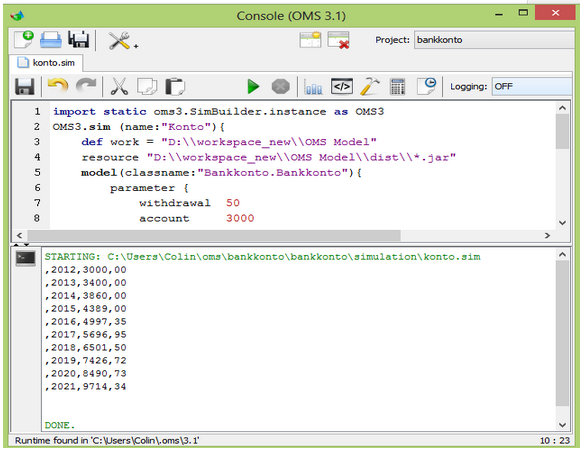
\includegraphics[width=0.7\textwidth]{pics/oms/Figure9.png}
	\caption{Result after running the model “bank account”
 \label{fig:Result_Bank_Account}}	
\end{figure}
\par
OMS also provides diagram visualization features for the simulation results for better understanding and evaluation. The following figure shows the diagram of the status changes of the bank account of different years.
\begin{figure}[h]
	\centering
	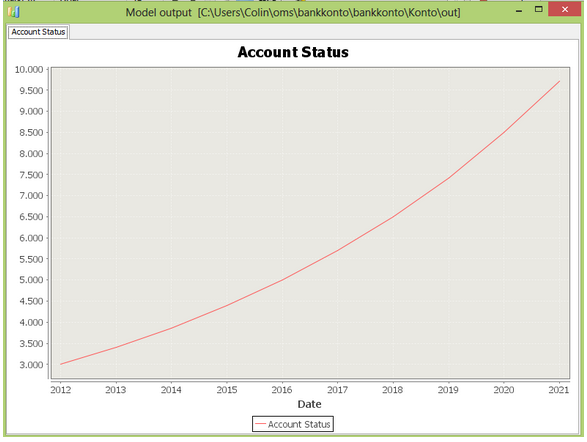
\includegraphics[width=0.7\textwidth]{pics/oms/Figure10.png}
	\caption{Visualization of the status of a bank account
 \label{fig:Visualization_Bank_Account}}	
\end{figure}
The new version of the OMS framework 3.1 supports multiple threading. Each OMS3 component will be executed in a separate thread, which is managed by the framework runtime. Thread communication happens when data flow from the “@Out” field of one component to the “@In” field of another component is carried out. The component will wait until all its necessary inputs are present and satisfied, then it starts to execute. Since modern computers are equipped with multi-core processors, the multi-threading feature will greatly make use of the power of the processors to improve the performance of the framework.
\par
\subsubsection{Advantages of OMS}
\par
The OMS framework provides the following benefits for model developers: [5]
\begin{enumerate}
\item The OMS framework enables efficient transfer of technology, because of the  integration of various software tools in one platform. Due to the common modeling platform and common user interface, the OMS will reduce the start-up time of model development and lower training costs of users.

\item The OMS framework reduces the costs of developing new software technologies. With OMS, model developers can put scientific knowledge into packages as modules in OMS to build new customized software packages at a small fraction of costs.

\item Model developers are able to apply the most suitable science to a specific problem. The OMS provides various software tools for model developers. The most appropriate modules for each individual natural problem and situation will be chosen.

\item The OMS framework enhances productivity of researchers and scientists. Model developers now focus on the science module implementation, other than graphical user interface, deployment, etc, which helps to increase the productivity and quality.

\end{enumerate}
\subsubsection{Disadvantages of OMS}
\par
Although the OMS framework provides various advantages for model developers, it also faces some difficulties. [5]
\begin{enumerate}
\item Model developers always lack of motivation to share model code, for example, the component libraries of environmental processes, environmental models, etc. Therefore, model developers have to build their own modules repositories or contribute to the OMS module library, so that they are available for other model developers to do further developments.

\item It is hard to predict whether a modular coding structure will be accepted or not. It will take much time for model developers to pay attention to the module design, especially the input and output requirements, module structure, meta data description, and proper use of annotations. In this way, the quality and usability of the module will be guaranteed.

\item Willingness to share data sets also affects the usability of the OMS framework. The data sets mentioned here are input or output of a model, for example, data for a range of natural resource processes covering different climatic and physio graphic regions across the world. Without these data sets, it is hard to reuse an existing model, since the data is important for comparison and evaluation. Without proper comparison and evaluation, further development of the existing model is almost impossible.

\item Furthermore, it is hard to transplant models, which are developed with the OMS framework, to other framework platforms. The interoperation ability of the OMS framework is not good enough, to make the models also run on other platforms flawlessly.

\end{enumerate}









